\scanpage{23}
\mspage{43}
\figure{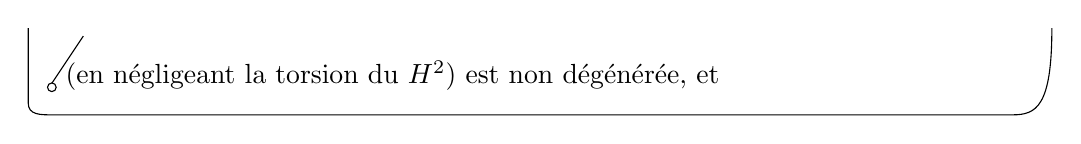
\begin{tikzpicture}[x=1cm,y=1cm]
\node[anchor=west] at (.35,0) {\inserted{(en négligeant la torsion du $H^2$) est non dégénérée, et}};
\draw (0,.6) -- (0,-.35) .. controls (0,-.5) and (.15,-.5) .. (.3,-.5) -- (12.5,-.5) .. controls (12.8,-.5) and (13,-.4) .. (13,.6);
\draw (.3,-.15) circle (.055);
\draw (.3,-.1)--(.7,.5);
\end{tikzpicture}}
\[
H^4(X,\underline Z_{\ell}[2])\simeq\underline Z_{\ell}.
\]
\deleted{D'après \unsure{il est}} Cette forme\figure{\begin{tikzpicture}[baseline=-.3ex,x=.4cm,y=.4cm]\draw (0,0) circle (.07);\draw (.03,.07)--(.5,.9);\end{tikzpicture}} induit sur $\operatorname{NS}(X)\otimes_{\underline Z}\underline Z_{\ell}$ la forme bilinéaire déduite de la \uline{forme intersection} sur $\operatorname{NS}(X)$, provenant de la multiplicité
\margin{$\times$}
globale d'intersections de diviseurs sur $X$ \inserted{[15]} \deleted{\unsure{?}}. D'après
\margin{$\times$}
MATSUSAKA \inserted{[27]}, cette dernière forme est non dégénérée. Tensorisant alors la suite exacte (8.7) par $\underline Q_{\ell}$, on trouve que $T_{\ell}(\operatorname{Br}^{\deleted{\unsure{\prime}}}(X))\otimes_{\underline Z_{\ell}}\underline Q_{\ell}$ \uline{s'identifie canoniquement à l'orthogonal de} $\operatorname{NS}(X)\otimes_{\underline Z_{\ell}}\underline Q_{\ell}$ \uline{dans} $H^2(X,\underline Q_{\ell}[1])$, \uline{et que le cup-produit définit sur cet espace une forme quadratique non dégénérée.}
L'interprétant comme une forme quadratique sur $T_{\ell}(\operatorname{Br}^{\deleted{\unsure{\prime}}}(X))$ à valeurs dans $\underline Q_{\ell}$, (et tenant compte que le cup-produit induit même une autodualité de $H^2/\mathrm{torsion}$) on trouve aisément que cette forme est à valeurs dans $\underline Z_{\ell}$ si et seulement si le discriminant de la forme intersection sur $\operatorname{NS}(X)/\mathrm{torsion}$ est une unité $\ell$-adique - condition qui est vérifiée donc pour presque tous les nombre premiers $\ell$ \deleted{\unsure{-}}, et que dans ce cas on trouve une autodualité de $T_{\ell}(\operatorname{Br}^{\deleted{\unsure{\prime}}}(X))$.

\inserted{8.3.} Ce résultat ne concerne essentiellement que la partie divisible $\operatorname{Br}'(X)^0$ du groupe de Brauer cohomologique. On peut également donner une relation de dualité concernant le \deleted{\unsure{gour|grou}} groupe fini $\operatorname{Br}'(X)/\operatorname{Br}'(X)^0$, qui grâce à la suite exacte de Kummer (BR II 3.1) s'explicite comme
\[
\tag{8.8}\operatorname{Br}'(X)/\operatorname{Br}'(X)^0\simeq H^2(X,\mu_{\ell^\infty})/H^2(X,\mu_{\ell^\infty})^0,
\]
(compte tenu que $\operatorname{Pic}(X)\otimes\underline Q_{\ell}/\underline Z_{\ell}=\operatorname{NS}(X)\otimes\underline Q_{\ell}/\underline Z_{\ell}$ est divisible). Utilisant (8.3) pour $i=3$, on trouve donc
\[
\tag{8.9}\operatorname{Br}'(X)/\operatorname{Br}'(X)^0\simeq\operatorname{Tors}H^3(X,\underline Z_{\ell}[1]),
\]
\inserted{(}valable indépendamment des hypothèses particulières \deleted{\unsure{faites}} \inserted{posées} au début de l'alinéa précédent pour $X$. Lorsque celles-ci sont vérifiées, alors les relations de dualité, bien connues dans le cas classique, et qui résultent aisément \figure{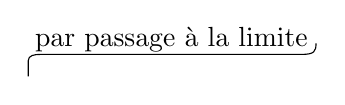
\begin{tikzpicture}[baseline=(p.base),x=1cm,y=1cm]
\node[inner sep=0pt,anchor=west] (p) at (0,0) {\inserted{par passage à la limite}};
\draw ([xshift=-.08cm,yshift=-.30cm]p.south west) -- ([xshift=-.08cm,yshift=-.10cm]p.south west) .. controls ([xshift=-.08cm,yshift=-.03cm]p.south west) and ([yshift=-.02cm]p.south west) .. ([xshift=.08cm,yshift=-.02cm]p.south west) -- ([xshift=-.08cm,yshift=-.02cm]p.south east) .. controls ([xshift=.08cm,yshift=-.02cm]p.south east) and ([xshift=.10cm,yshift=.02cm]p.south east) .. ([xshift=.10cm,yshift=.12cm]p.south east);
\end{tikzpicture}} des résultats de dualité [SGAA $\overline{\underline{\mathrm{XIX}}}$\quad] pour des
\margin{$\times$}
\mspage{22}
